\FloatBarrier
\section{Utility tolerance, case floors, and exchange uncertainty}
\label{app:v8}
These additional analyses are retrospective and use the existing paired fits, frozen candidate scores and previously evaluated periods. Their specifications, input hashes and code hashes were recorded before the new computations. The scientific choices were informed by earlier results and review; this chronology is not prospective preregistration. No new models or external data were introduced. All grid settings and no-choice conditions are retained in the accompanying source, under \texttt{evidence/revision\_v8\_*} and \texttt{evidence/revision\_v9\_*}.

\subsection{Conditional uncertainty of the observed exchanges}
\label{app:v8-exchange}
For every original relative-.95 policy, define $Q=\Delta d/(-\Delta c)$ from exposure-choice minus case-choice coverage. We use 4,000 item-cluster draws (seed 20260915), sharing multiplicities across arms and head cells and retaining each item's stores and dates. Every case-loss denominator is positive; the smallest is 13.5332 points. Tables~\ref{tab:v8-exchange} and \ref{tab:v8-exchange-difference} report all ratios and complete-minus-censored differences, with central 95\% and four-contrast-adjusted percentile summaries.
\begin{table}[t]\centering\small
\caption{All eight original policy exchanges $\Delta d/(-\Delta c)$ at each arm\textquotesingle s primary relative cap. Central 95\% percentile intervals use 4,000 item resamples and condition on fits, caps, thresholds and choices. All case-loss denominators are positive in every draw; these intervals omit calibration reselection.}\label{tab:v8-exchange}
\begin{tabular}{llrl}\toprule
Arm & Heads $e/w$ & Exchange & Conditional interval\\\midrule
Censored & 220/220 & 0.1764 & [0.1155, 0.2472] \\
Censored & 660/220 & 0.2040 & [0.1374, 0.2811] \\
Censored & 220/660 & 0.2130 & [0.1508, 0.2835] \\
Censored & 660/660 & 0.2034 & [0.1393, 0.2781] \\
Complete & 220/220 & 0.6150 & [0.4829, 0.7779] \\
Complete & 660/220 & 0.3316 & [0.2548, 0.4302] \\
Complete & 220/660 & 0.2835 & [0.2181, 0.3621] \\
Complete & 660/660 & 0.3061 & [0.2316, 0.4019] \\
\bottomrule\end{tabular}\end{table}

\begin{table}[t]\centering\small
\caption{Complete-minus-censored exchange differences, with shared item multiplicities across arms. The four-contrast intervals use empirical .00625/.99375 quantiles. Adjustment gives approximate conditional summaries, not simultaneous population certification or a causal effect of censoring.}\label{tab:v8-exchange-difference}
\begin{tabular}{lrll}\toprule
Heads $e/w$ & Difference & Pointwise interval & Four-contrast interval\\\midrule
220/220 & 0.4387 & [0.3577, 0.5403] & [0.3398, 0.5750] \\
660/220 & 0.1277 & [0.0912, 0.1658] & [0.0841, 0.1762] \\
220/660 & 0.0705 & [0.0459, 0.0951] & [0.0400, 0.1015] \\
660/660 & 0.1027 & [0.0709, 0.1377] & [0.0626, 0.1479] \\
\bottomrule\end{tabular}\end{table}

All four matched-head point differences and adjusted intervals are positive at their respective arm-relative caps; this is not a causal efficiency comparison. The complete 220/220 Ratio branch has $Q=.615044$ [.482931,.777873]. Substituting its existing Descending candidate while retaining Excess gives -35.1632 case/+10.0836 exposure points and $Q=.286766$ [.218574,.368456]. This is a fixed-candidate comparison. These intervals condition on fitted models, caps, thresholds and choices; they omit calibration reselection and common store/calendar shocks. No selection-inclusive exchange distribution or bimodality has been established.

\subsection{Margins at stricter relative caps}
\label{app:v8-strict}
All 30 calibration candidates at relative caps .85/.90/.95 are reconstructed for both 220/220 arms. At .85/.90, Descending is infeasible in both arms, so its Ratio margin is undefined. Complete-sales Ratio exceeds feasible runner-up Mixed by 4.0141/3.4327 pp. Censored .85 selects Mixed with Ratio infeasible; .90 selects Ratio by 2.5829 pp (Table~\ref{tab:v8-strict}). Complete .85 Ratio has minimum case coverage 35.0362\%, close to the .35 floor. These finite-menu observations do not isolate error-head value or establish robustness to a stricter floor.
\begin{table}[t]\centering\scriptsize
\caption{Original 220/220 calibration menus at three relative caps. Margins are minimum-calibration-exposure differences in pp. R/D denote Ratio/Descending. Undefined comparisons are shown as -- when a candidate is infeasible; zero accepted mass is not a feasible competing policy. The strongest feasible other candidate is Mixed at .85/.90 and Descending at .95.}\label{tab:v8-strict}
\begin{tabular}{lrrlllrr}\toprule
Arm & Cap factor & Eligible & Winner & R feasible & D feasible & R--D & R--Other\\\midrule
Censored & 0.85 & 2 & Mixed & no & no & -- & -- \\
Censored & 0.90 & 3 & Ratio & yes & no & -- & 2.5829 \\
Censored & 0.95 & 4 & Descending & yes & yes & -0.5442 & -0.5442 \\
Complete & 0.85 & 3 & Ratio & yes & no & -- & 4.0141 \\
Complete & 0.90 & 3 & Ratio & yes & no & -- & 3.4327 \\
Complete & 0.95 & 4 & Ratio & yes & yes & 0.0270 & 0.0270 \\
\bottomrule\end{tabular}\end{table}


\FloatBarrier
\subsection{Exposure allowances: alternatives and exact selection intervals}
\label{app:v8-tolerance}
Equation~\eqref{eq:menu-choice} remains the primary audit rule. Equation~\eqref{eq:tolerance} is a retrospective alternative: it changes utility, retaining the original thresholds, eligibility and case choice. The illustrative .5 pp allowance and grid $\{0,.1,.25,.5,1\}$ pp were recorded before the v8 computation, informed by the earlier audit. All 40 choices were frozen before evaluation; the allowance is neither an operational recommendation nor a confidence threshold. Tables~\ref{tab:v8-tolerance-grid}--\ref{tab:v8-tolerance-frequency} retain the complete grid, eight-cell results and frequencies.
\begin{figure}[t]\centering
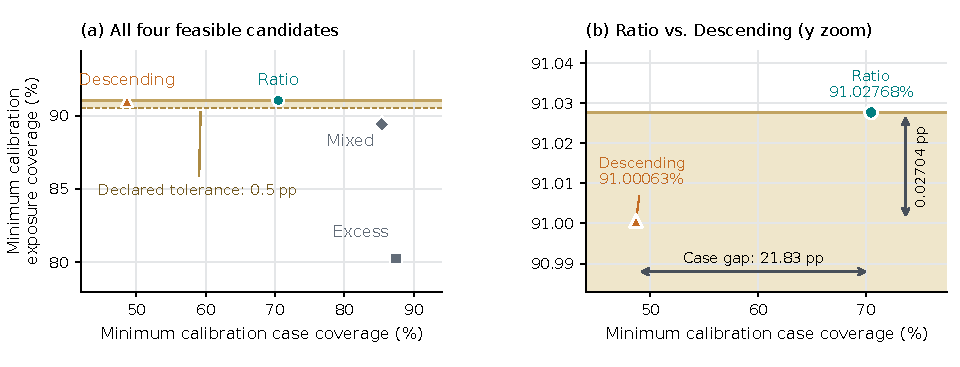
\includegraphics[width=\linewidth]{revision_v8_neartie.pdf}
\caption{Complete-sales 220/220 calibration candidates; Error is infeasible. Minimum case and exposure coverage are taken separately over A/B. The right panel magnifies the exposure axis. Shading marks the illustrative .5-point utility allowance, clipped by the zoom; it is not a confidence interval. Ratio and Descending are close in exposure but far apart in cases.}\label{fig:near-tie}
\end{figure}
\begin{table}[t]\centering\scriptsize
\caption{Complete tolerance grid: exposure-rule choices with original thresholds held fixed. Column values are exposure-coverage allowances in pp. Case choices remain Excess throughout. This is an explicit utility preference, not a confidence region. All candidate metrics and 40 condition outcomes are retained in the accompanying results.}\label{tab:v8-tolerance-grid}
\begin{tabular}{lllllll}\toprule
Arm & Heads & 0 & .1 & .25 & .5 & 1.0\\\midrule
Censored & 220/220 & Descending & Descending & Descending & Descending & Ratio \\
Censored & 660/220 & Descending & Descending & Descending & Descending & Descending \\
Censored & 220/660 & Descending & Descending & Descending & Descending & Ratio \\
Censored & 660/660 & Descending & Descending & Descending & Descending & Descending \\
Complete & 220/220 & Ratio & Ratio & Ratio & Ratio & Ratio \\
Complete & 660/220 & Descending & Descending & Descending & Ratio & Ratio \\
Complete & 220/660 & Descending & Ratio & Ratio & Ratio & Ratio \\
Complete & 660/660 & Descending & Descending & Descending & Ratio & Ratio \\
\bottomrule\end{tabular}\end{table}

\begin{table}[t]\centering\scriptsize
\caption{All eight cells at the declared .5 pp exposure tolerance. Case choice remains Excess. Cal. cost is the minimum-calibration-exposure concession; Later gain/cost compare the tolerance-selected exposure policy with the original exposure choice. Final columns compare the new exposure choice with the unchanged case choice. The .621 pp Later cost in complete 660/220 exceeds the calibration allowance.}\label{tab:v8-tolerance}
\begin{tabular}{llllrrrr}\toprule
Arm & Heads & Original/new & Cal. cost & Later $c$ gain & Later $d$ cost & $\Delta c$ & $\Delta d$\\\midrule
Censored & 220/220 & Descending/Descending & 0.000 & 0.00 & -0.000 & -39.95 & 7.05 \\
Censored & 660/220 & Descending/Descending & 0.000 & 0.00 & -0.000 & -40.66 & 8.29 \\
Censored & 220/660 & Descending/Descending & 0.000 & 0.00 & -0.000 & -37.94 & 8.08 \\
Censored & 660/660 & Descending/Descending & 0.000 & 0.00 & -0.000 & -40.04 & 8.14 \\
Complete & 220/220 & Ratio/Ratio & 0.000 & 0.00 & -0.000 & -15.81 & 9.72 \\
Complete & 660/220 & Descending/Ratio & 0.388 & 24.11 & 0.621 & -10.41 & 10.83 \\
Complete & 220/660 & Descending/Ratio & 0.094 & 13.62 & 0.251 & -21.23 & 9.63 \\
Complete & 660/660 & Descending/Ratio & 0.360 & 19.00 & 0.476 & -15.98 & 10.23 \\
\bottomrule\end{tabular}\end{table}


Table~\ref{tab:v8-tolerance} compares the alternative with both the unchanged case choice and the original exposure choice. One evaluation exposure cost is .6208 pp, exceeding .5; the allowance only bounds the calibration concession.

\paragraph{Analytic intervals.}
For an eligible Ratio candidate $R$, let $D=\max_j\bar d_j$ and $P_j=(\bar c_j,\bar d_j,-j)$, where $j$ is the fixed tie order. Its exact selection interval is
\[
 [L_R,U_R)=\left[D-\bar d_R,\;\min_{j:P_j>_{\rm lex}P_R}(D-\bar d_j)\right).
\]
The upper bound is infinite if there is no higher-priority candidate; the interval is empty if $U_R\leq L_R$ or Ratio is ineligible. The lower bound admits Ratio; the upper bound admits a candidate that defeats it. We check \emph{all} eligible competitors, not just Descending.

For complete-sales 220/220, 660/220, 220/660 and 660/660, the intervals are approximately [0,1.634053), [.388433,2.508229), [.093843,1.646188) and [.360002,2.252009) pp. Mixed supplies every upper endpoint. Their intersection is approximately [.388433,1.634053), containing the conservatively rounded [.39,1.63] pp interval. Thus .5 is not an isolated grid value, but this descriptive interval does not justify selecting a utility from the desired family.

The same 200 complete-reference redesign draws all have nonempty Ratio intervals. Lower-endpoint empirical 2.5/50/97.5 percentiles are 0/0/.479234 pp; upper-endpoint percentiles are .596676/1.643270/3.088298 pp. Exactly 194 contain .5. Bike has 192 nonempty intervals and eight empty ones because Mixed already dominates when Ratio becomes eligible. Nonempty lower endpoints are zero, and upper percentiles are .188918/1.436880/3.550370 pp; .5 belongs to 172 of \emph{all} 200 intervals. These are conditional descriptive endpoint distributions, not confidence bounds. No four-head joint redesign distribution exists in the archive.
\begin{table}[t]\centering\scriptsize
\caption{Exposure-rule frequency (\%) after applying each tolerance to the same 200 threshold-redesign draws from the earlier audit. Fitted scores, cap, $T$, and draw identities are unchanged. The .5 pp rule makes Ratio more frequent in the complete-sales reference and less frequent in Bike; a wider band need not monotonically favor Ratio.}\label{tab:v8-tolerance-frequency}
\begin{tabular}{llrrrrrr}\toprule
Setting & Tolerance pp & Error & Excess & Mixed & Ratio & Desc. & None\\\midrule
Complete 220/220 & 0.00 & 0.0 & 0.0 & 0.0 & 51.5 & 48.5 & 0.0 \\
Complete 220/220 & 0.10 & 0.0 & 0.0 & 0.0 & 69.0 & 31.0 & 0.0 \\
Complete 220/220 & 0.25 & 0.0 & 0.0 & 0.5 & 83.5 & 16.0 & 0.0 \\
Complete 220/220 & 0.50 & 0.0 & 0.0 & 1.5 & 97.0 & 1.5 & 0.0 \\
Complete 220/220 & 1.00 & 0.0 & 0.0 & 16.0 & 83.5 & 0.5 & 0.0 \\
Bike & 0.00 & 0.0 & 0.0 & 4.0 & 96.0 & 0.0 & 0.0 \\
Bike & 0.10 & 0.0 & 0.0 & 4.5 & 95.5 & 0.0 & 0.0 \\
Bike & 0.25 & 0.0 & 0.0 & 8.0 & 92.0 & 0.0 & 0.0 \\
Bike & 0.50 & 0.0 & 0.0 & 14.0 & 86.0 & 0.0 & 0.0 \\
Bike & 1.00 & 0.0 & 0.0 & 34.5 & 65.5 & 0.0 & 0.0 \\
\bottomrule\end{tabular}\end{table}

The source retains all draw intervals and candidate records under \texttt{evidence/revision\_v9\_epsilon/}. Exact-rational breakpoint checks and independent floating-point replay validate the intervals. The implementation's $10^{-12}$ coverage-fraction comparison tolerance moves positive boundaries by only $10^{-10}$ pp. No new fits, threshold searches, resampling draws or evaluation outcomes enter this interval analysis.

\FloatBarrier
\subsection{A-design screening, floors, and exposure allowances}
\label{app:v8-floor}
The floor audit uses .35/.40/.45, four head pairs and five rankings (60 conditions), with reporting/design caps .6326834234/.6010492522 and fitted arrays fixed. Largest feasible whole-tie A thresholds are screened on B using 4,000 item resamples (seed 20260912), at tails .05/60 and .05/20. All 40 nonempty conditions pass (16/12/12 by floor). Exact A utility determines choices before rereading Later data.

Raising the floor either retains the largest risk-feasible threshold or makes its family infeasible; a smaller threshold cannot restore lost case coverage. Descending accepts 35.0483/35.0938\% on A, so even .36 excludes it. Floors .40/.45 select Excess/Ratio throughout, with Later contrasts -26.78 to -16.81 case/+11.59--12.72 exposure points (Table~\ref{tab:v8-floor-main}). Ratio at 220/660 accepts only 45.0574\% on A, limiting extrapolation. The source retains the full 60-condition screen and 24 selected records (48 with both adjustments), including duplicated policies, in \texttt{evidence/revision\_v8\_floor/}; the detailed v8 table files are also retained.

\begin{table}[t]\centering\small
\caption{Complete-sales A-design/B-screen floor sensitivity, all four head pairs per row. Ranges show Later exposure-choice minus case-choice coverage (pp), not confidence intervals. $U_{60}$ is the largest approximate upper risk summary among selected conditions, adjusted over all 60 candidate conditions. Fixed reporting cap is .632683; the same selection occurs under the inherited 20-candidate adjustment.}\label{tab:v8-floor-main}
\begin{tabular}{llllr}\toprule
Floor & Case/exposure rules & $\Delta c$ range & $\Delta d$ range & Max. $U_{60}$\\\midrule
0.35 & Excess/Descending & [-36.39, -35.83] & [12.77, 14.29] & 0.62802 \\
0.40 & Excess/Ratio & [-26.78, -16.81] & [11.59, 12.72] & 0.62756 \\
0.45 & Excess/Ratio & [-26.78, -16.81] & [11.59, 12.72] & 0.62756 \\
\bottomrule\end{tabular}\end{table}


\paragraph{Composing the tolerance rule with screening.}
We now apply the same interval formula to the existing B-passing candidates, using A utility. At floor .35, Descending exceeds Ratio in exposure by 1.083012/1.846934/1.247238/1.597532 pp in the four head settings above. Mixed supplies all upper bounds. The common interval is approximately [1.846934,3.741367) pp: allowances 0/.5/1 retain Descending throughout, whereas 2 selects Ratio throughout. At floors .40/.45, the common Ratio interval is [0,2.494129) pp, so all four tested allowances select Ratio. Both screen-family adjustments agree. All conditions and breakpoint checks are retained in \texttt{evidence/revision\_v9\_screen\_tolerance/}.

The near-tie result for the original joint-A/B design does not extend to this stricter A-only design. Under the illustrative .5 pp allowance, its family switch is caused by the floor restriction; a larger declared concession supplies a different route. This establishes neither a universal allowance nor the causal effect of changing the design cap alone. Selected Later upper summaries remain approximate and fit-conditional: the largest $U_{60}=.62802431<r$, but .05/60 in 4,000 draws leaves only about 3.3 draws in the tail. Union risk and prospective generalization are not evaluated.
